%% Le lingue utilizzate, che verranno passate come opzioni al pacchetto babel. Come sempre, l'ultima indicata sarà quella primaria.
%% Se si utilizzano una o più lingue diverse da "italian" o "english", leggere le istruzioni in fondo.
\def\thudbabelopt{english}
%% Valori ammessi per target: bach (tesi triennale), mst (tesi magistrale), phd (tesi di dottorato).
%% Valori ammessi per aauheader: '' (vuoto -> nessun header Alpen Adria Univeristat), aics (Department of Artificial Intelligence and Cybersecurity), informatics (Department of Informatics Systems). Il nome del dipartimento è allineato con la versione inglese del logo UniUD.
%% Valori ammessi per style: '' (vuoto -> stile moderno), old (stile tradizionale).
\documentclass[target=bach,aauheader=,style=]{thud}

%% --- Informazioni sulla tesi ---
%% Per tutti i tipi di tesi
% Scommentare quello di interesse, o mettete quello che vi pare
\course{Informatica}
%\course{Internet of Things, Big Data e Web}
%\course{Matematica}
%\course{Comunicazione Multimediale e Tecnologie dell'Informazione}
\title{Automatic Nuclei Segmentation and Counting in Histopathology Images with U-Net}
\author{Pantanali Riccardo}
\supervisor{Prof.\ Della Mea Vincenzo}
\cosupervisor{Dott.ssa \ Teresa Pace}
\tutor{Guido Necchi}
%% Campi obbligatori: \title, \author e \course.
%% Altri campi disponibili: \reviewer, \tutor, \chair, \date (anno accademico, calcolato in automatico), \rights
%% Con \supervisor, \cosupervisor, \reviewer e \tutor si possono indicare più nomi separati da \and.
%% Per le sole tesi di dottorato:
\phdnumber{313}
\cycle{XXVIII}
\contacts{Via della Sintassi Astratta, 0/1\\65536 Gigatera --- Italia\\+39 0123 456789\\\texttt{http://www.example.com}\\\texttt{inbox@example.com}}

%% --- Pacchetti consigliati ---
%% pdfx: per generare il PDF/A per l'archiviazione. Necessario solo per la versione finale
\usepackage[a-1b]{pdfx}
%% hyperref: Regola le impostazioni della creazione del PDF... più tante altre cose. Ricordarsi di usare l'opzione pdfa.
\usepackage[pdfa]{hyperref}
\usepackage{tikz}
\usepackage{subcaption}
\usepackage{amsmath}
\usepackage{float}
%% tocbibind: Inserisce nell'indice anche la lista delle figure, la bibliografia, ecc.

%% --- Stili di pagina disponibili (comando \pagestyle) ---
%% sfbig (predefinito): Apertura delle parti e dei capitoli col numero grande; titoli delle parti e dei capitoli e intestazioni di pagina in sans serif.
%% big: Come "sfbig", solo serif.
%% plain: Apertura delle parti e dei capitoli tradizionali di LaTeX; intestazioni di pagina come "big".

\begin{document}
\maketitle

%% Dedica (opzionale)
\begin{dedication}
	Al mio cane,\par per avermi ascoltato mentre ripassavo le lezioni.
\end{dedication}

%% Ringraziamenti (opzionali)
\acknowledgements
Sed vel lorem a arcu faucibus aliquet eu semper tortor. Aliquam dolor lacus, semper vitae ligula sed, blandit iaculis leo. Nam pharetra lobortis leo nec auctor. Pellentesque habitant morbi tristique senectus et netus et malesuada fames ac turpis egestas. Fusce ac risus pulvinar, congue eros non, interdum metus. Mauris tincidunt neque et aliquam imperdiet. Aenean ac tellus id nibh pellentesque pulvinar ut eu lacus. Proin tempor facilisis tortor, et hendrerit purus commodo laoreet. Quisque sed augue id ligula consectetur adipiscing. Vestibulum libero metus, lacinia ac vestibulum eu, varius non arcu. Nam et gravida velit.

%% Sommario (opzionale)
\abstract
Nunc ac dignissim ipsum, quis pulvinar elit. Mauris congue nec leo ornare lobortis. Nulla hendrerit pretium diam nec lobortis. Nullam aliquam laoreet nisl, sit amet facilisis lectus accumsan ut. Duis et elit hendrerit metus venenatis condimentum. Integer id eros molestie, interdum leo sit amet, aliquet metus. Integer fermentum tristique magna, vel luctus neque rhoncus vel. Ut hendrerit et quam et semper. Mauris egestas, odio sed aliquet luctus, magna orci euismod odio, vitae lacinia tellus tellus non lectus. Aliquam urna neque, porta et mattis aliquam, congue sit amet lorem. In ultrices augue sit amet ante vehicula, vitae rhoncus turpis auctor. Donec porta scelerisque eros, at mollis enim imperdiet ut. 

%% Indice
\tableofcontents

%% Lista delle tabelle (se presenti)
%\listoftables

%% Lista delle figure (se presenti)
%\listoffigures

%% Corpo principale del documento
\mainmatter

%% Parte
%% La suddivisione in parti è opzionale; solitamente sono sufficienti i capitoli.
%\part{Parte}

%% Capitolo
\chapter{Dataset}
The analysis of nuclear features in histopathology images has long been recognized as a crucial aspect of cancer research and diagnosis. The part that seems like a bottleneck is the limited size of the most publicy available dataset for nuclei segmentation and classification, and often suffering from sparse labelling or sampling bias.\\
To address this limitations, Gamper et al. (2019) 
\cite{gamper2019pannuke,gamper2020pannuke} introduce and extended PanNuke, an open pan-cancer a semi-automatically obtained for nuclei instance segmentation and classification dataset.

%% Sezione
\section{Materials}
PanNuke is created through multiple model combinantions with already existing public data for nuclei classification$/$segmentation. To produce the proposed dataset have been sampled patches randomly extracted from a Whole Slide Image (WSI), using 19 different TCGA tissue types and other internal dataset for prostate, colon, ovarian, breast and oral tissue.\\
In total, 455 visual field were collected, of which 312 were randomly sampled from more than 200.000 H\&E-stained WSI, using a random approach to chose the patch allowed the authors to address the selection bias present in available public dataset. To overcome the scarity of ground truth and the unreliability of manual labeling, have been adopted a three stream approach regarding segmentation, classification and detection models.\\
For the segmentation stream, the authors used the Kumar \cite{article} dataset and CPM17 \cite{vu2018methodssegmentationclassificationdigital} dataset. For the detection stream, additional images were extracted from TCGA and the Bone Morrow \cite{10.1007/978-3-319-24574-4_33} dataset  . The classification stream, the nuclei were labeled using MonuSeg, ColonNuclei, SPIE cellularity challenge data, and the Nuclei Attribute dataset, ensuring a diverse set of nuclear categories.\\

\begin{table}[ht]
\centering
\caption{PanNuke Nuclei Categories from initial datasets}
\label{tab:pannuke_init}
\resizebox{\textwidth}{!}{%
\begin{tabular}{lrrrrrrr}
\hline\hline
 & \multicolumn{7}{c}{\textbf{PanNuke Nuclei Categories}} \\
\cline{2-8}
\textbf{Dataset} & \textbf{Neoplastic} & \textbf{Non-Neo Epithelial} & \textbf{Inflammatory} & \textbf{Connective} & \textbf{Dead} & \textbf{Non-Nuclei} & \textbf{Total} \\
\hline
MoNuSeg          & 5,927 &   836 & 1,698 &   906 &   0 &   0 &   9,367 \\
Colon Nuclei     & 4,685 & 7,544 & 6,003 & 4,468 & 2,547 &   0 &  25,247 \\
BreastPathQ      & 9,802 &     0 & 2,139 &     0 &   0 &   0 &  11,941 \\
Nuclei Attribute &     0 &     0 &     0 &     0 &   0 & 500 &     500 \\
\hline
\textbf{Total}   &20,414 & 8,380 & 9,840 & 5,374 & 2,547 & 500 & 47,055 \\
\hline\hline
\end{tabular}%
}
\end{table}
\section{Method}
The authors followed three pathways to abtaind the validated dataset. These three pathways are segmentation, detection and classification. Using the CNN trained on patches extracted from the datasets in Table 1, they classified all the labeled nuclei part of the above datasets mentioned, which were then verified by a team of pathologists and classified by the PanNuke categories.\\
After, they took 2,000 patches from more than 20,000 WSI in 19 tissues obtained from a TCGA.
The models predictions were evaluated in terms of uncertainty, like a clear misclassification. The expert pathologists re-annotated these difficult cases, and the corrected annotations were used to retrain the models. 
\begin{figure}[h] % l'opzione [h] cerca di posizionare l'immagine "here"
    \centering
    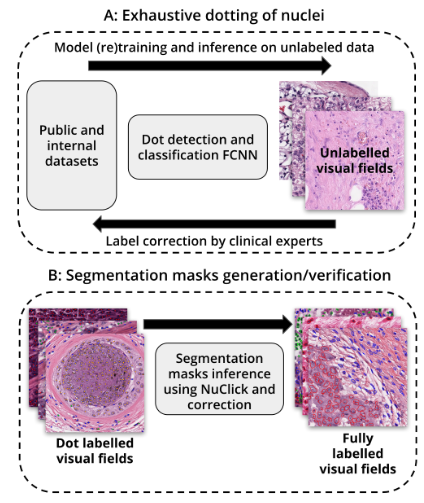
\includegraphics[width=0.45\textwidth]{imgs/pannuke_annotations.png}
    \caption{Questa è la didascalia dell'immagine}
    \label{fig:esempio}
\end{figure}
Then proceed to Part A of annotation process Figure 1.1. After a total of 7 iterations of the process, pathologists would evaluate and re-label the detected and classified nuclei.\\
To generate the segmentation masks they use NuClick \cite{jahanifar2019nuclick}, that brings an accurate segmentation mask from a single point. 
\section{Class Distribution}
\label{sec:classdistribution}
In evarage, most nuclei types that have been provided belongs in all tissues considered in PanNuke.
\begin{figure}[h]
  \centering
  \begin{minipage}{0.45\textwidth}
    \centering
    \includegraphics[width=\linewidth]{imgs/class_distributionù.png}
    \caption{Didascalia 1}
  \end{minipage}\hspace{2cm}
  \begin{minipage}{0.3\textwidth}
    \centering
    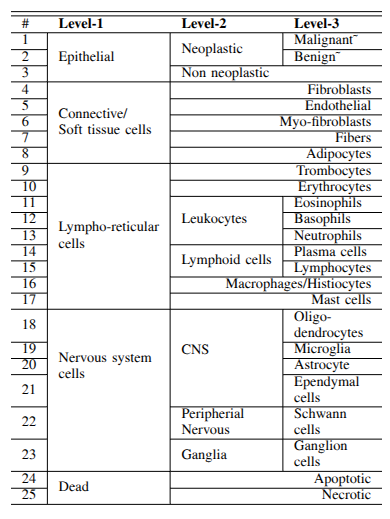
\includegraphics[width=\linewidth]{imgs/class_tab.png}
    \caption{Didascalia 2}
  \end{minipage}
\end{figure}
PanNuke defines nuclei into five categories, tab 1.3: \textbf{Neoplastic} includes any type of tumor, malignant or benign, therefore includes carcinomas, sarcomas, melanomas, lymphomas, etc. Those tumors are originate from different cell types: carcnimoas from epithelial; sarcomas from lymphoid cells etc.\\
\textbf{Non-neoplastic} covers everything else, thus different categories from normal to inflammatory, metaplastic, degenerative, etc.\\
\textbf{Connective} cells have the potential to become tumors.\\
\textbf{Inflammatory} cells include macrophage and lymphoid, unlike connective cells, inflammatory cells cannot become plastic.\\
\textbf{Dead cells} can arise from neoplastic or non-neoplastic.\\

In figure 1.2 we can observe that the distribution of the total nuclei count per tissue and per class changes between tissue types. We observe that there is a strong imbalance reflects the biological prevalence of cell types in histopathology slides that will become a challenge for deep learning models. In particular, the nucleis categoriesed dead are rare, therefore will be difficult to segment and classify.\\
Overall, the class distribution prove that PanNuke offers both large quantities of common cell types and valuable examples of underrepresented nuclei, reaching a realistic dataset that mirrors the cases that could present in clinical practice.

\section{Dataset Statistics}
The PanNuke dataset provides nuclei annotations across 19 tissue types, with each nucleus labeled according to one of five clinically relevant categories. The dataset contains 189,744 nulei annotated at the instance level.\\
For the purpose of this work, only neoplastic nuclei where considered. This choice was motivated by the specific objective of our study, which focused on identifying and counting malignant cells. In practice, the ground truth masks were converted in bianry masks, where each positive pixel belong to a neoplastic nucleo and the remaining pixels were just merged with the background.\\

By restricting the dataset to neoplstic nuclei, the resulting distribution is imbalanced compared to the full PanNuke schema.
%% Fine dei capitoli normali, inizio dei capitoli-appendice (opzionali)
\chapter{Methodology}
\section{Workflow}

The workflow of the proposed project follows a typical deep learning pipeline for nuclei segmentation, adapted to the specific goal of detecting and counting neoplastic nuclei in histopathology images.

First, raw images and their corresponding annotations are pre-processed in order to generate the inputs required by the model. In particular, original instance masks provided in PanNuke are converted into binary masks representing the presence of neoplastic nuclei, and distance maps are computed to capture spatial relationships between adjacent nuclei.

The core of the system is based on a U-Net \cite{DBLP:journals/corr/RonnebergerFB15} architecture extended with two output heads. This multi-head workflow allows the model to simultaneously learn pixel-wise classification and spatial structural information, ensuring better generalization and robustness in the task of nuclei segmentation and counting.
\subsection{Tool and environment}
The development of the project required specific tools for model training and the pipeline execution. In this section will be presented the main software tools and the specific hardware components of the development enviroment. The entire project have been develop in Python 3.12.\\

\noindent\textbf{Hardware environment}\\

\noindent The whole pipeline have been execute on a PC, which has the following components:
\begin{itemize}
    \item \textbf{CPU}: AMD Ryzen 5 9600X, 6 core / 12 thread
    \item \textbf{GPU}: NVIDIA RTX 3080 Ti 11 global
    \item \textbf{RAM}: 32 GB DDR 5 6000 MHz
    \item \textbf{Operative System}: Linux Ubuntu (64 bit)
    \item \textbf{Caching CPU}: L3 38 MiB
\end{itemize}
This enviroment has garanted enough camputational calc for the model training.
\subsection{Pipiline}
The pipeline was developed to ensure the reproducibility of the workflow: from the pre processing to the automatic models evaluation. 
\section{Pre processing}
Preprocessing is a fundamental step, as it adapts the raw PanNuke data to the specific objective of segmenting and counting neoplastic nuclei. Since, the main goal is segment and count the neoplastic nuclei, this requires transforming the instance-level annotations into binary masks, as well as generating distance maps that help to separete the different cluster of nucleis.\\
In addition, the original RGB images were processed using blu colormaps, hematoxylin-extracted H\&E channels and grayscale, to understand how various input affect segmentation performance.
\subsection{Dataset files}
\label{sec:datafiles}
The raw PanNuke dataset is organized into three folder inside each folder there are 3 files .npy:

\begin{enumerate}
    \item \textbf{types.npy}: contains the categorical label of each nucleus. Since this project does not address nuclear classification, this file is not used.
    
    \item \textbf{mask.npy}: contains $N$ images, each with a size of $256 \times 256$ pixels and 6 channels.  
    The first five channels correspond to the instance maps of the nuclear categories described in Section~\ref{sec:classdistribution}.  
    Specifically, the first channel encodes the instance map of neoplastic nuclei in the $n$-th image, the second channel the instance map of non-neoplastic epithelial nuclei, and so on.  
    The sixth channel is a binary mask that includes all nuclei, regardless of category, in the $n$-th image.
    
    \item \textbf{image.npy}: contains $N$ images, each with a size of $256 \times 256$ pixels and 3 channels, representing the original RGB images.
\end{enumerate}
\begin{center}
    \begin{tikzpicture}
        \node (img1) {\includegraphics[height=3cm]{imgs/class_distributionù.png}};

        \node (img2) at (img1.south east){\includegraphics[height=3cm]{imgs/class_distributionù.png}};
    \end{tikzpicture}
\end{center}
\subsection{Image Preprocessing}
The image preprocessing was developed to evaluate the impact of different input on the main task. 
The raw dataset provides RGB images described in Section~\ref{sec:datafiles}. 
From these images, additional channels were derived to highlight nuclear structures and assess whether color information affects models performances. 

Specifically, four different input variants were considered:

\begin{itemize}
    \item \textbf{RGB}: the original $256 \times 256$ image RGB.
    \item \textbf{Hematoxylin (H\&E)}: images obtained by color deconvolution, where the hematoxylin channel is extracted to emphasize nuclear morphology \cite{ruifrok2001quantification}.
    \item \textbf{Blue colormap}: a transformed representation where intensity values are mapped to a blue color scale, enhancing contrast between nuclei and background.
    \item \textbf{Grayscale}: single-channel images representing intensity only, without color information.
\end{itemize}
By preprocessing the dataset into these four modalities, the experimental pipeline allows a direct comparison of how different color representations influence segmentation accuracy. 
\begin{figure}[h!]
    \centering
    % Riga 1
    \begin{subfigure}{0.45\textwidth}
        \centering
        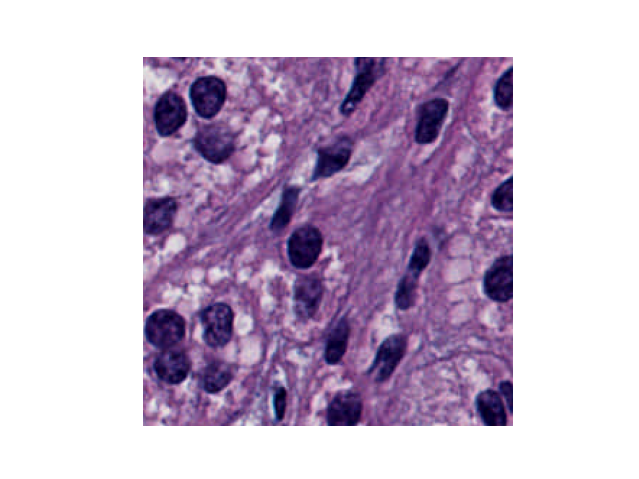
\includegraphics[width=\linewidth]{imgs/RGB.png}
        \caption{RGB}
    \end{subfigure}
    \hspace{0.2cm}
    \begin{subfigure}{0.45\textwidth}
        \centering
        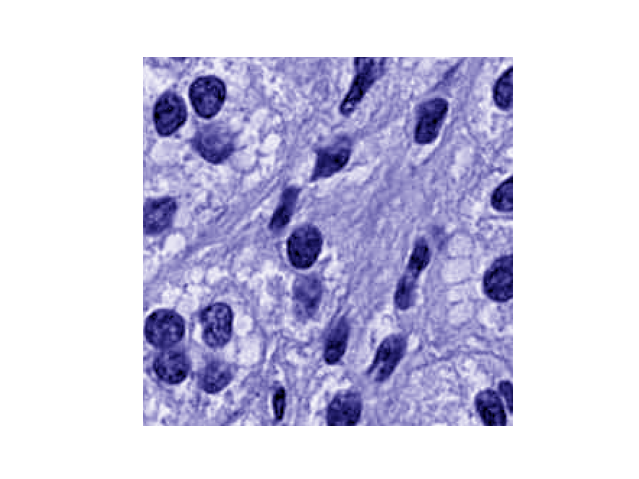
\includegraphics[width=\linewidth]{imgs/HE.png}
        \caption{Hematoxylin}
    \end{subfigure}
    
    \vspace{0.4cm} % spazio verticale fra le righe
    
    % Riga 2
    \begin{subfigure}{0.45\textwidth}
        \centering
        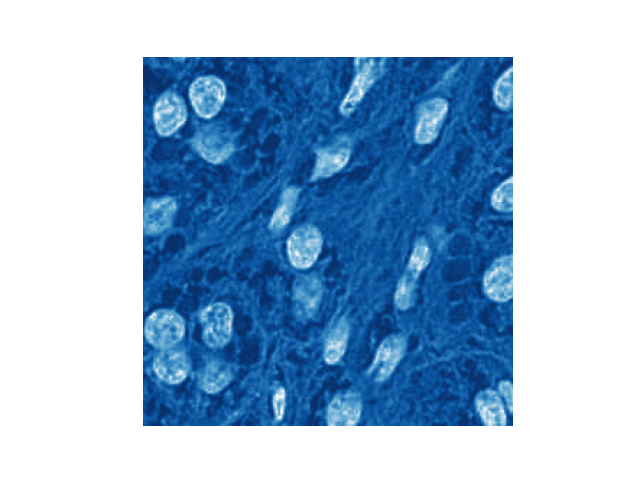
\includegraphics[width=\linewidth]{imgs/Blu.png}
        \caption{Blu channel}
    \end{subfigure}
    \hspace{0.2cm}
    \begin{subfigure}{0.45\textwidth}
        \centering
        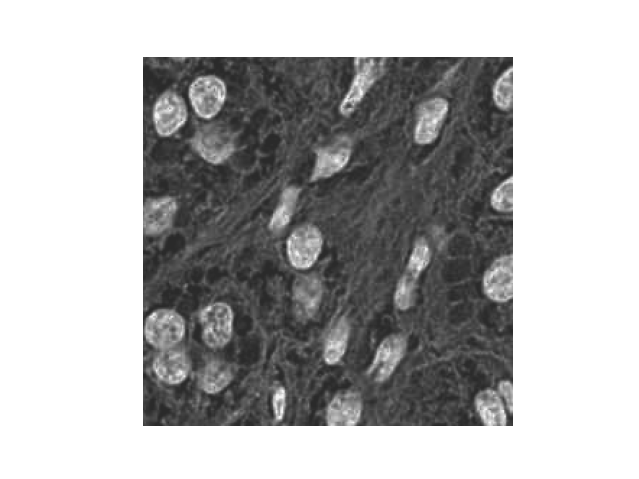
\includegraphics[width=\linewidth]{imgs/Gray.png}
        \caption{Gray scale}
    \end{subfigure}
    
    \caption{Each type of color representations used}
    \label{fig:quattro_immagini}
\end{figure}

\subsection{Mask Generation}
In the PanNuke datasets there are different files described in Section~\ref{sec:datafiles}, for this work will be use only a part of them. The task is to study the segmentation and counting of neoplastic cells. Therefore, the generation of binary masks and distance maps pivot on that goal.\\

\noindent\textbf{Binary masks}\\
From the file \texttt{masks.npy}, have been extracted the channel corresponding to the neoplastic cells. The image extracted is $256 \times 256$ and provide as an instance map, where every individual cell is assigned a unique label (e.g., 1, 2, 3,\dots). Subsequently, to obtain a binary mask, all non-zero pixel in the instance map are mapped to 1, while background pixels remain 0. The instance map $I$, the corresponding binary mask $B$:
\begin{center}
$
B(i) = 
\begin{cases}
1 & \text{if } I(i) > 0 \\
0 & \text{if } I(i) = 0
\end{cases}
$
\end{center}
where $i$ denote a pixel location. Before being used each binary mask is converted into a three-channel trugh the function \texttt{\_mask\_to\_3ch}:
\begin{itemize}
    \item \textbf{Body}: Each positive pixel is assigned to a nucleus.
    \item \textbf{Background}: Each positive pixel not belonging to any nucleus, therefore is part of the background.
    \item \textbf{Border}: a contour around each nucleus, obtained by applying a morphological erosion to the binary mask and the substracting the eroded mask from the original.
\end{itemize}
This three-channel encoding brings to distinguish nuclear region from background, therefore increase the segmentation performance.\\
\begin{figure}[H] % l'opzione [h] cerca di posizionare l'immagine "here"
    \centering
    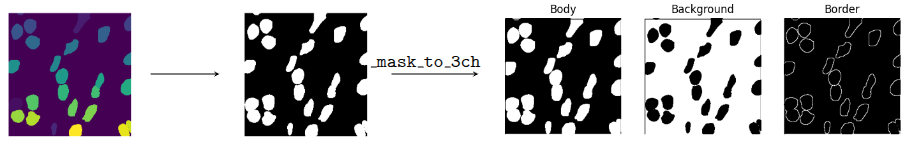
\includegraphics[width=1\textwidth]{imgs/binarymask_transform.png}
    \caption{Transformation from instance map to binary mask with 3 channels}
    \label{fig:esempio}
\end{figure}
\noindent\textbf{Distance maps}\\
\subsection{Data Augmentation}
\section{Model Architecture}
\section{Loss Function}
\section{Training Strategy}
\section{Post Processing}
\section{Evaluation Metrics}

\appendix

%\part{Appendici}

\chapter{Titolo della prima appendice}
Sed purus libero, vestibulum ut nibh vitae, mollis ultricies augue. Pellentesque velit libero, tempor sed pulvinar non, fermentum eu leo. Duis posuere eleifend nulla eget sagittis. Nam laoreet accumsan rutrum. Interdum et malesuada fames ac ante ipsum primis in faucibus. Curabitur eget libero quis leo porttitor vehicula eget nec odio. Proin euismod interdum ligula non ultricies. Maecenas sit amet accumsan sapien.

%% Parte conclusiva del documento; tipicamente per riassunto, bibliografia e/o indice analitico.
\backmatter

%% Riassunto (opzionale)
%\summary
%Maecenas tempor elit sed arcu commodo, dapibus sagittis leo egestas. Praesent at ultrices urna. Integer et nibh in augue mollis facilisis sit amet eget magna. Fusce at porttitor sapien. Phasellus imperdiet, felis et molestie vulputate, mauris sapien tincidunt justo, in lacinia velit nisi nec ipsum. Duis elementum pharetra lorem, ut pellentesque nulla congue et. Sed eu venenatis tellus, pharetra cursus felis. Sed et luctus nunc. Aenean commodo, neque a aliquam bibendum, mauris augue fringilla justo, et scelerisque odio mi sit amet diam. Nulla at placerat nibh, nec rutrum urna. Donec ut egestas magna. Aliquam erat volutpat. Phasellus vestibulum justo sed purus mattis, vitae lacinia magna viverra. Nulla rutrum diam dui, vel semper mi mattis ac. Vestibulum ante ipsum primis in faucibus orci luctus et ultrices posuere cubilia Curae; Donec id vestibulum lectus, eget tristique est.

%% Bibliografia (praticamente obbligatoria)
\bibliographystyle{plain_\languagename}%% Carica l'omonimo file .bst, dove \languagename è la lingua attiva.
%% Nel caso in cui si usi un file .bib (consigliato)
\bibliography{thud}
%% Nel caso di bibliografia manuale, usare l'environment thebibliography.
%% Per l'indice analitico, usare il pacchetto makeidx (o analogo).

\end{document}

--- Istruzioni per l'aggiunta di nuove lingue ---
Per ogni nuova lingua utilizzata aggiungere nel preambolo il seguente spezzone:
    \addto\captionsitalian{%
        \def\abstractname{Sommario}%
        \def\acknowledgementsname{Ringraziamenti}%
        \def\authorcontactsname{Contatti dell'autore}%
        \def\candidatename{Candidato}%
        \def\chairname{Direttore}%
        \def\conclusionsname{Conclusioni}%
        \def\cosupervisorname{Co-relatore}%
        \def\cosupervisorsname{Co-relatori}%
        \def\cyclename{Ciclo}%
        \def\datename{Anno accademico}%
        \def\indexname{Indice analitico}%
        \def\institutecontactsname{Contatti dell'Istituto}%
        \def\introductionname{Introduzione}%
        \def\prefacename{Prefazione}%
        \def\reviewername{Controrelatore}%
        \def\reviewersname{Controrelatori}%
        %% Anno accademico
        \def\shortdatename{A.A.}%
        \def\summaryname{Riassunto}%
        \def\supervisorname{Relatore}%
        \def\supervisorsname{Relatori}%
        \def\thesisname{Tesi di \expandafter\ifcase\csname thud@target\endcsname Laurea\or Laurea Triennale\or Dottorato\fi}%
        \def\tutorname{Tutor aziendale}%
        \def\tutorsname{Tutor aziendali}%
    }
